\begin{figure}[!tbp]\centering
\begin{minipage}[c]{0.46\textwidth}\centering
% PROVENANCE: run=d2-gpu-r2-4b-labour-v1 trial=labour_vi_v1-l1_rerank-s42-LVN-009-a1 (ledger steps and token counts copied from trials.jsonl)
\begin{tikzpicture}[font=\scriptsize,x=1cm,y=1cm,
  st/.style={draw=blue!55!black,fill=blue!8,rounded corners=2pt,align=left,inner sep=3pt,text width=7.0cm,line width=0.6pt},
  qq/.style={st,fill=black!5,draw=black!60},
  rs/.style={st,fill=black!10,draw=black!70},
  fl/.style={-{Stealth[length=4.5pt,width=4pt]},line width=0.7pt}]
\node[qq] (q) at (0,0) {\textbf{Question} (translated): under Decree 293/2025, what is the hourly minimum wage in region IV?};
\node[st,below=0.32cm of q] (a) {\textbf{1~search.} Query ``Nghị định 293/2025/NĐ-CP mức lương tối thiểu giờ vùng IV''; BM25 + TF-IDF give 20 candidates, the reranker keeps 5; Article 3 of the decree is ranked first. \emph{1,574 tokens in, 105 out.}};
\node[st,below=0.32cm of a] (b) {\textbf{2~read.} Full text of Article 3 of Decree 293/2025. \emph{2,921 in, 166 out.}};
\node[st,below=0.32cm of b] (c) {\textbf{3~answer.} ``17,800 VND per hour'', quote ``Vùng IV 3.700.000 17.800'' from Article 3. \textbf{Citation verifier: accepted, 0 repairs.} \emph{3,623 in, 211 out.}};
\node[rs,below=0.32cm of c] (r) {\textbf{Outcome:} answered with a verified citation; 8,118 tokens in, 482 out in total. The answer equals the benchmark's reference answer.};
\draw[fl] (q) -- (a); \draw[fl] (a) -- (b); \draw[fl] (b) -- (c); \draw[fl] (c) -- (r);
\end{tikzpicture}\\[2pt]{\small (a) Trace of LuatCheck (4B controller, verifier and reranker on).}
\end{minipage}\hfill
\begin{minipage}[c]{0.52\textwidth}\centering
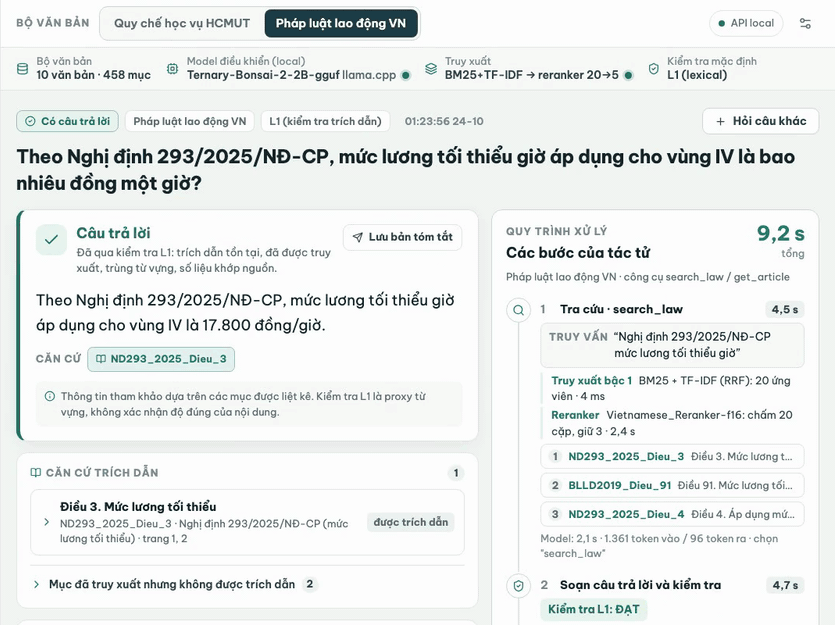
\includegraphics[width=\linewidth]{images/demo_answer.png}\\[2pt]{\small (b) Web interface, same question.}
\end{minipage}
\caption{(a) One completed trial from the evaluation (a labour-law question about the hourly minimum wage, seed 42). (b) The web interface answering the same question, showing the answer, citation verifier status, highlighted source section and step timeline.}\label{fig:trace}
\end{figure}
